\documentclass[10pt,pdf,utf8,russian,aspectratio=169]{beamer}
\usepackage[T2A]{fontenc}
\usepackage[english,russian]{babel}
\usepackage{subfig}
%
% Choose how your presentation looks.
%
% For more themes, color themes and font themes, see:
% http://deic.uab.es/~iblanes/beamer_gallery/index_by_theme.html
%
\mode<presentation>
{
  \usetheme{Boadilla}      % or try Darmstadt, Madrid, Warsaw, ...
  \usecolortheme{seagull} % or try albatross, beaver, crane, ..

  \usefonttheme{structurebold}  % or try serif, structurebold, ...
  \setbeamertemplate{navigation symbols}{}
  \setbeamertemplate{caption}[numbered]
} 

\captionsetup[subfloat]{labelformat=empty}
\title[Сложность модели]{Сложность моделей глубокого обучения}
\author{Бахтеев Олег}
\institute{МФТИ}
\date{12.04.2017}

\begin{document}

\begin{frame}
  \titlepage
\end{frame}

% Uncomment these lines for an automatically generated outline.
\begin{frame}{План}
  \tableofcontents
\end{frame}

\section{Сложность модели}
\begin{frame}{Сложность модели: зачем?}
\begin{figure}
  \centering
  \subfloat[Устойчивость моделей при возмущении выборки]{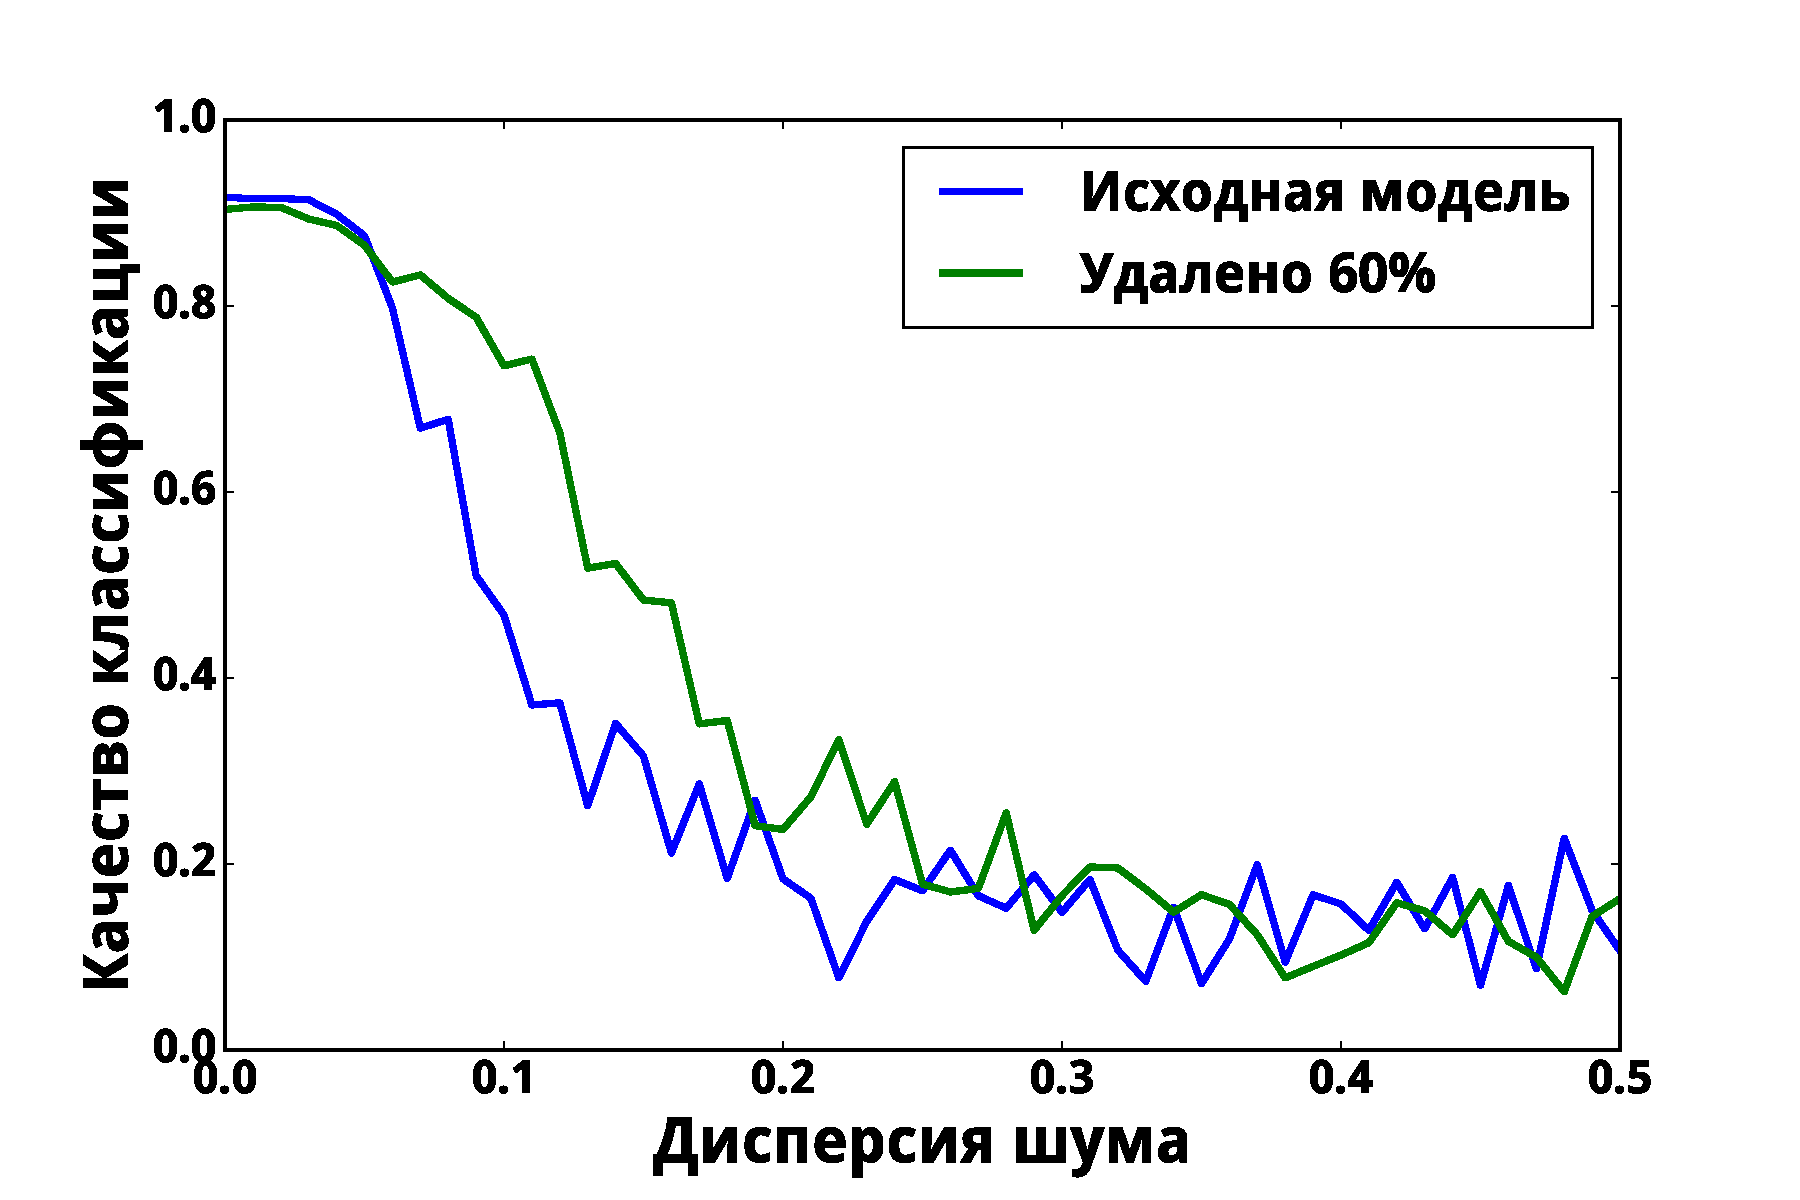
\includegraphics[width=0.4\textwidth]{noise.pdf}} 
 \subfloat[Качество классификации при удалении параметров]{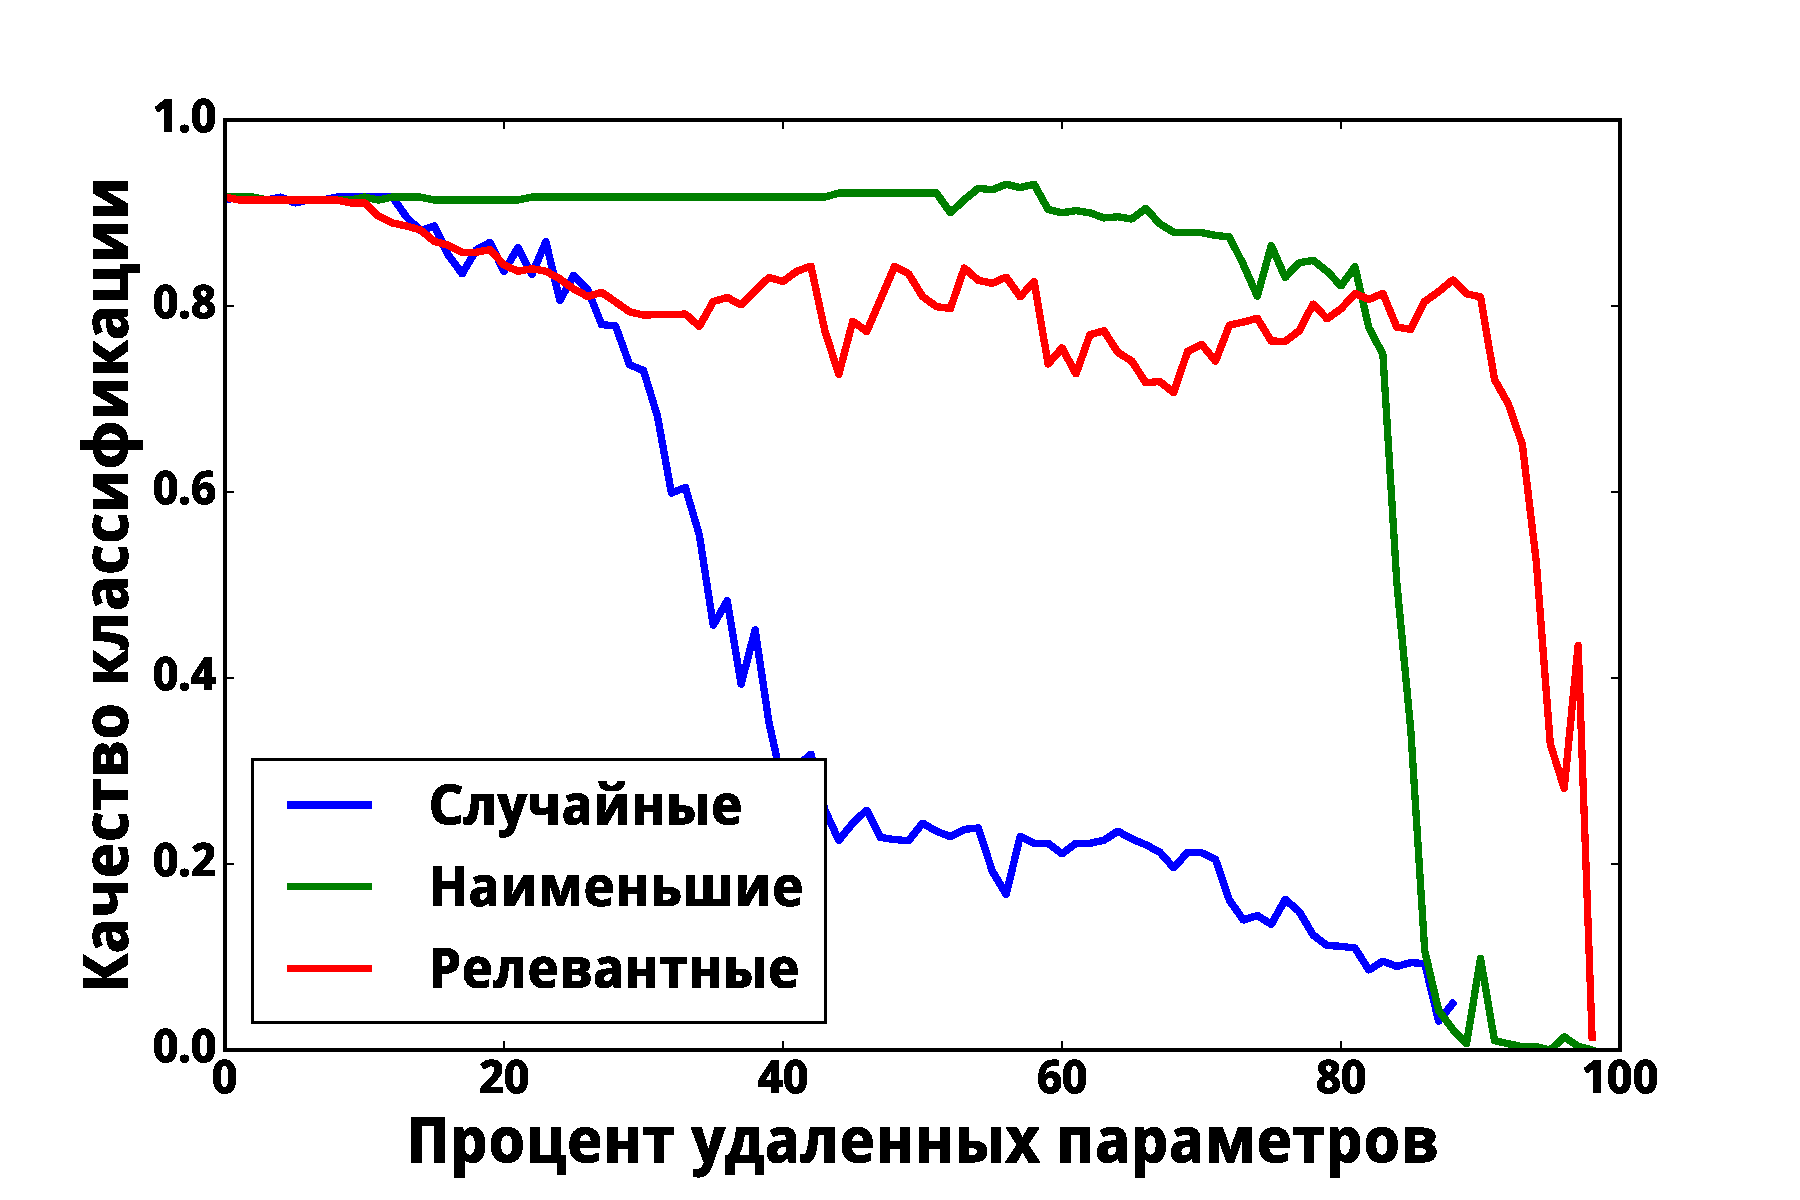
\includegraphics[width=0.4\textwidth]{pruning.pdf}}
\label{fig:1}\qquad

\end{figure}


\end{frame}


\begin{frame}{Принцип минимальной длины описания}
\[
\text{MDL}(\mathbf{f}, \mathbf{X}) = L(\mathbf{f}) + L(\mathbf{X}|\mathbf{f}),
\]
где $\mathbf{f}$ --- модель, $\mathbf{X}$ --- выборка, $L$ --- длина описания в битах.
\\
\[
\text{MDL}(\mathbf{f}, \mathbf{X}) \sim L(\mathbf{f}) + L(\mathbf{w}^*| \mathbf{f}) + L(\mathbf{X}|\mathbf{w}^*, \mathbf{f}),
\]
$\mathbf{w}^*$ --- оптимальные параметры модели.\\

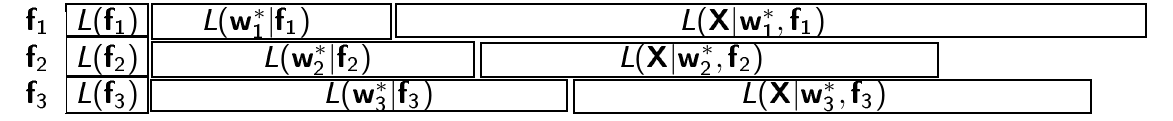
\includegraphics[width=\textwidth]{./mdl.png}
%$\mathbf{f}_1: L(\mathbf{f}_1)\qquad L(\mathbf{w}_1^*| \mathbf{f}_1) \qquad \qquad \qquad \qquad \qquad	\qquad L(\mathbf{X}|\mathbf{w}_1^*, \mathbf{f}_1) $\\
%$\mathbf{f}_2: L(\mathbf{f}_2)\qquad \qquad L(\mathbf{w}_2^*| \mathbf{f}_2) \qquad \qquad \qquad \qquad L(\mathbf{X}|\mathbf{w}_2^*, \mathbf{f}_2) $\\
%$\mathbf{f}_3: L(\mathbf{f}_3)\qquad \qquad \qquad L(\mathbf{w}_3^*| \mathbf{f}_3) \qquad \qquad \qquad \qquad \qquad L(\mathbf{X}|\mathbf{w}_3^*, \mathbf{f}_3) $

\end{frame}

\begin{frame}{MDL и Колмогоровская сложность}
\textbf{Колмогоровская сложность} --- длина минимального кода для выборки на предварительно заданном языке.

\textbf{Теорема инвариантности}\\
Для двух сводимых по Тьюрингу языков колмогоровская сложность  отличается не более чем на константу, не зависяющую от мощности выборки.\\

\textbf{Отличия от MDL}:
\begin{itemize}
\item Колмогоровская сложность невычислима.
\item Длина кода может зависеть от выбранного языка. Для небольших выборок теорема инвариантности не дает адекватных результатов.
\end{itemize}
\end{frame}

\begin{frame}{Оптимальная универсальная модель MDL}
Пусть выборка $\mathbf{X}$ лежит в некотором конечном множестве $\mathbb{X}: \mathbf{X} \subset \mathbb{X}$.
%2.20
\[
\text{MDL}(\mathbf{f}, \mathbf{X}) = L(\mathbf{X}|\mathbf{w}^*(\mathbf{X}), \mathbf{f}) + \text{COMP}(\mathbf{f}),
\]
$$ L(\mathbf{X}|\mathbf{w}^*, \mathbf{f}) = -\text{log}p(\mathbf{X}|\mathbf{w}^*(\mathbf{X}), \mathbf{f}), \quad 
\text{COMP} = \text{log} \sum_{\mathbf{X}' \in \mathbb{X}} P(\mathbf{X}'|\mathbf{w}^*(\mathbf{X}'), \mathbf{f}).$$

В случае, если распределение $p(\mathbf{X}|\mathbf{w})$ принадлежит экспоненциальному семейству, оценка MDL совпадает с точностью до $o(1)$ с байесовской оценкой правдоподобия (``Evidence''):
\[
	p(\mathbf{X}|\mathbf{f}) = \int_\mathbf{w} p(\mathbf{X}|\mathbf{w})p(\mathbf{w}) d\mathbf{w},
\]
где $p(\mathbf{w})$ --- априорное распределение специанльного вида:
$$
	p(\mathbf{w}) = \frac{\sqrt{|J(\mathbf{w})|}}{\int_{\mathbf{w}'} \sqrt{|J(\mathbf{w'})|}d\mathbf{w'}},
$$
$J(\mathbf{w})$  --- информация Фишера.
\end{frame}	


\begin{frame}{Байесовый подход к сложности}
Правдоподобие модели (``Evidence''):
\[
	p(\mathbf{X}|\mathbf{f}) = \int_\mathbf{w} p(\mathbf{X}|\mathbf{w})p(\mathbf{w}|\mathbf{f}) d\mathbf{w}.
\]


\begin{figure}
  \centering
  \subfloat[Схема выбора модели по правдоподобию]{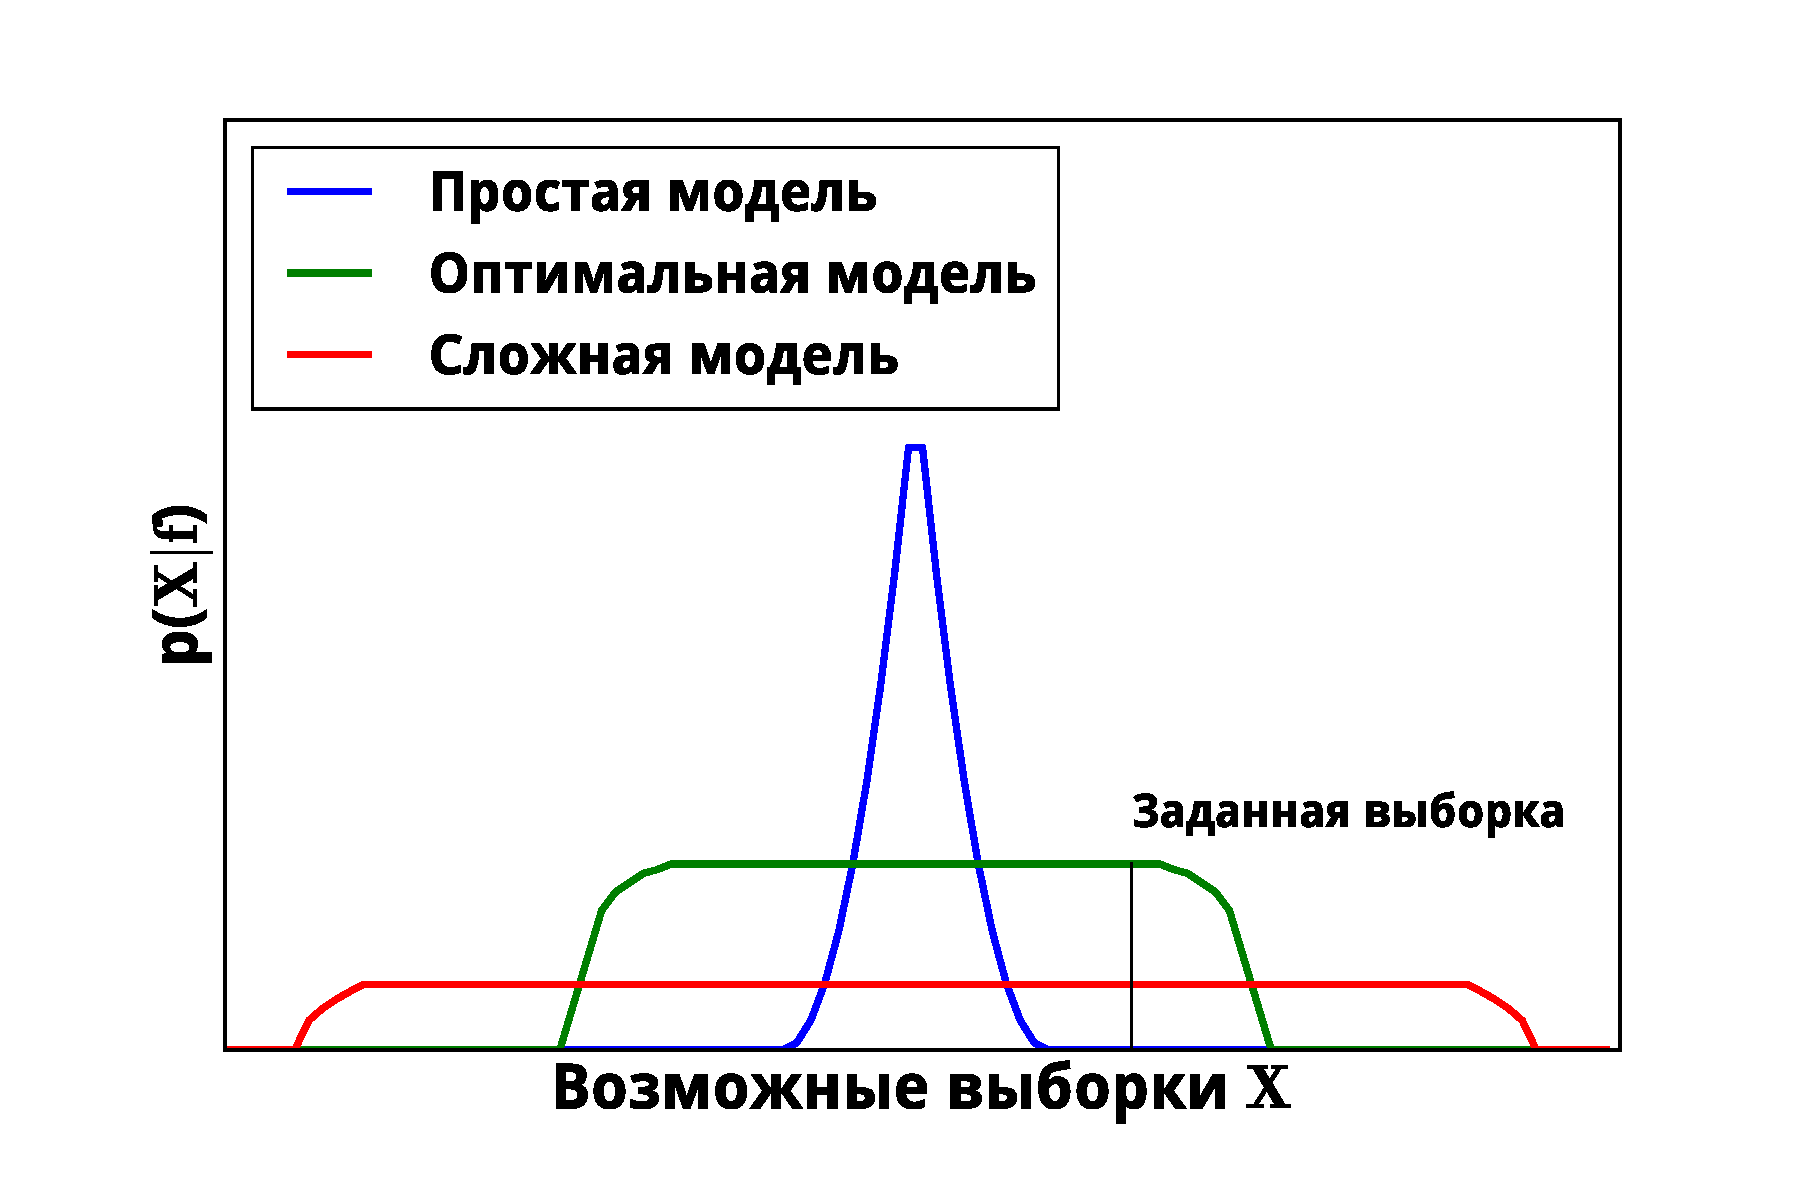
\includegraphics[width=0.4\textwidth]{evidence.pdf}} 
 \subfloat[Пример: полиномы]{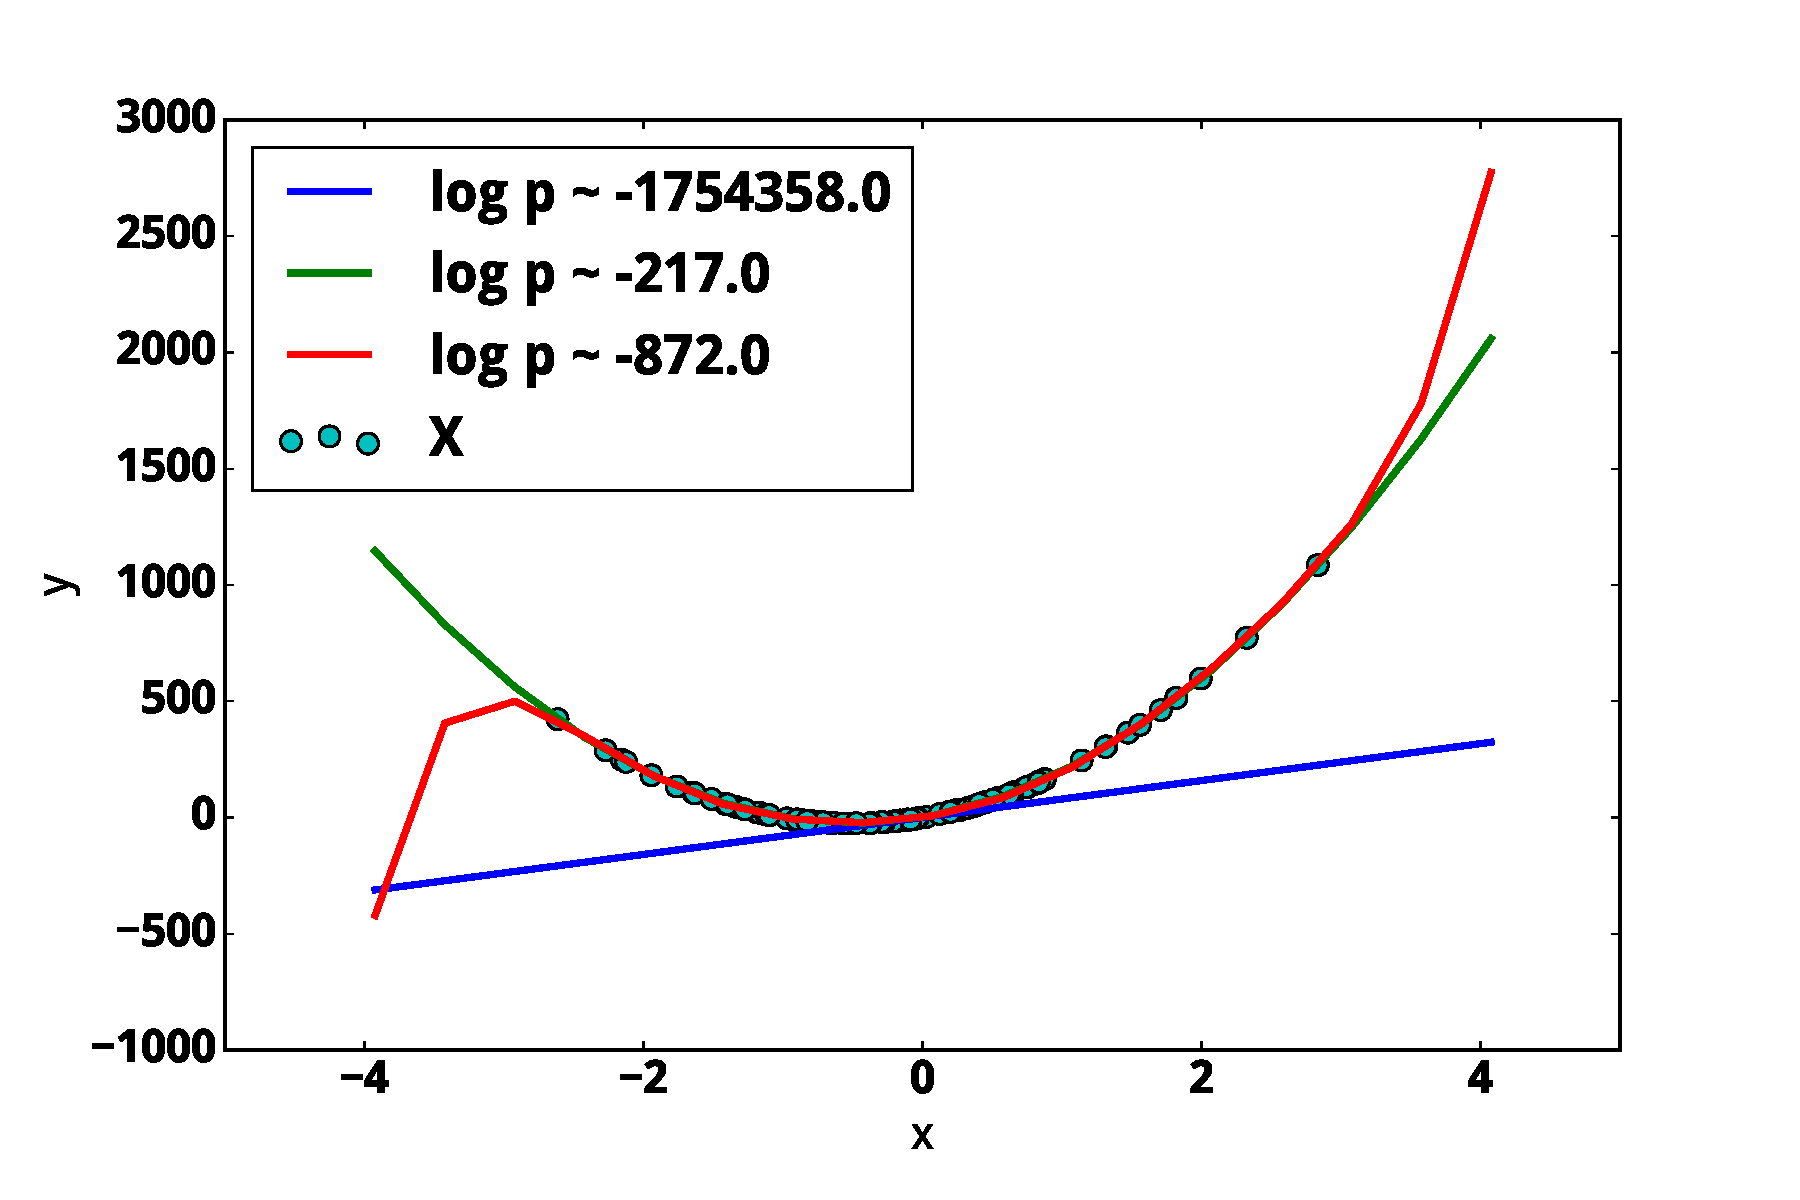
\includegraphics[width=0.4\textwidth]{example.pdf}}
\label{fig:1}\qquad

\end{figure}


\end{frame}

\begin{frame}{Evidence vs MDL}
\begin{tabular}{ c | c  }
  \hline			
  Evidence & MDL \\
  \hline  
Регуляризация признаков на основе априорных знаний &  - \\
  \hline  
Основывается на гипотезе о порождении\\ выборки & Минимизирует длину описания выборки\\ вне зависимости от их природы \\
  \hline  

\end{tabular}


\begin{figure}
  \centering
 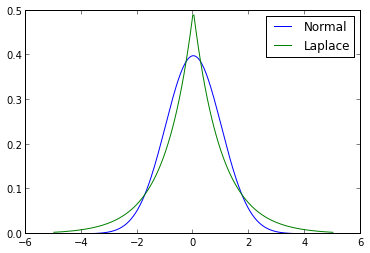
\includegraphics[width=0.4\textwidth]{laplace.png}
\label{fig:1}\qquad

\end{figure}
\end{frame}

\begin{frame}{Evidence vs Кросс-валидация}
Оценка Evidece:
\[
\text{log}~p(\mathbf{X}|\mathbf{f}) = \text{log}~p(\mathbf{x}_1|\mathbf{f}) + \text{log}~p(\mathbf{x}_2|\mathbf{x}_1, \mathbf{f}) + \dots +  \text{log}~p(\mathbf{x}_n|\mathbf{x}_1,\dots,\mathbf{x}_{n-1}, \mathbf{f}).
\]

Оценка leave-one-out:
\[
\text{LOU} = \mathsf{E} \text{log}~p(\mathbf{x}_n|\mathbf{x}_1,\dots,\mathbf{x}_{n-1}, \mathbf{f}).
\]

Кросс-валидация использует среднее значение последнего члена $p(\mathbf{x}_n|\mathbf{x}_1,\dots,\mathbf{x}_{n-1}, \mathbf{f})$ для оценки сложности. \\
Evidence учитывает \textbf{полную} сложность описания заданной выборки, определяющую предсказательную способность модели с самого начала.
\end{frame}

\begin{frame}{Методы получения оценок Evidence}
\begin{itemize}
\item{Аппроксимация методом Лапласа}\\
$$
	p(\mathbf{X}|\mathbf{f}) = \int_\mathbf{w} p(\mathbf{X}|\mathbf{w}) p(\mathbf{w}|\mathbf{f}) = \int_\mathbf{w} \text{exp}(-S(\mathbf{w}))	\sim  \text{exp}S(\hat{\mathbf{w}}) \int_\mathbf{w} \text{exp} (-\frac{1}{2}\Delta \mathbf{w}^\text{T} \nabla \nabla S(\hat{\mathbf{w}}) \Delta \mathbf{w} ).
$$

\item {Методы Монте-Карло}
$$
p(\mathbf{X}|\mathbf{f})  \sim \frac{1}{K}\sum_{\mathbf{w} \in \mathbf{W}} p(\mathbf{X}|\mathbf{w},\mathbf{f})p(\mathbf{w}|\mathbf{f}),
$$
$\mathbf{W}$ --- множество векторов параметров мощностью $K$.
\end{itemize}
\begin{figure}
  \centering
 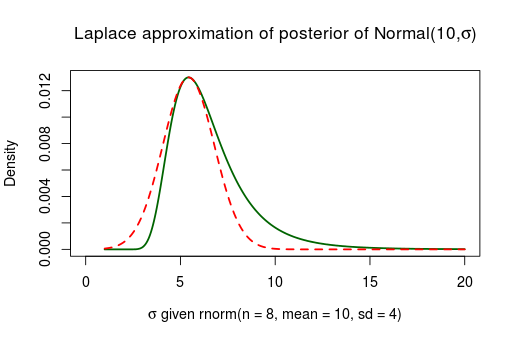
\includegraphics[width=0.4\textwidth]{laplace2.png}
\label{fig:1}\qquad	
\end{figure}
\end{frame}

\section{Вариационная нижняя оценка}
\begin{frame}{Вариационная оценка}
%http://www.orchid.ac.uk/eprints/40/1/fox_vbtut.pdf
\textbf{Вариационная оценка Evidence} --- метод нахождения приближенного значения аналитически невычислимого распределения $p(\mathbf{w}|\mathbf{X}, \mathbf{f})$ распределением $q(\mathbf{w}) \in \mathbf{Q}$. Получение вариационной нижней оценки обычно сводится к задаче минимизации
$$\text{KL}(q(\mathbf{w})||p(\mathbf{w}| \mathbf{X}))=
-\int_{\mathbf{w}} q(\mathbf{w}) \text{log}~\frac{p(\mathbf{w}| \mathbf{X})} {q(\mathbf{w})}d\mathbf{w}.
$$

\begin{figure}
  \centering
  \subfloat[Аппроксимация неизвестного распределения нормальным]{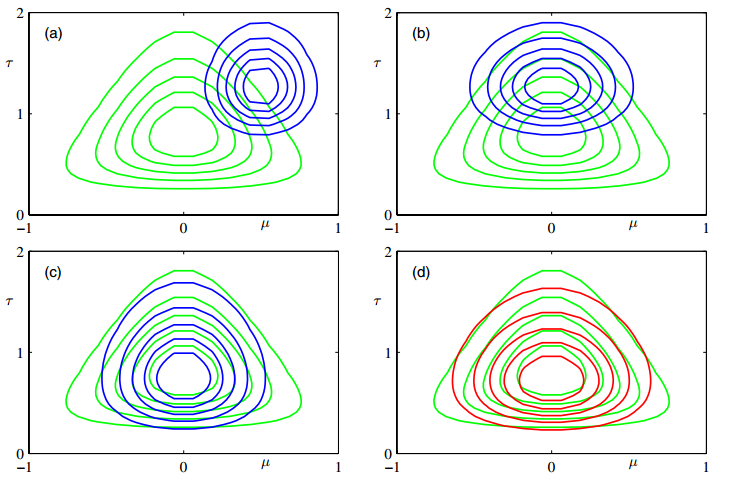
\includegraphics[width=0.35\textwidth]{omnomnom.png}} 
 \subfloat[Апроксимация Лапласа и вариационная оценка]{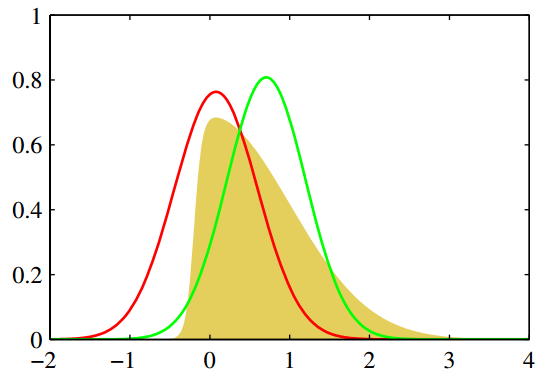
\includegraphics[width=0.35\textwidth]{laplace_vs_var.png}}
\label{fig:1}\qquad

\end{figure}

\end{frame}

\begin{frame}{Получение вариацонной нижней оценки}
$$
\text{log}~p(\mathbf{X}| \mathbf{f})  = \int_{\mathbf{w}} q(\mathbf{w})\text{log}~\frac{p(\mathbf{X},\mathbf{w}|\mathbf{f})}{q(\mathbf{w})}d\mathbf{w} + \text{D}_\text{KL}  (q(\mathbf{w})||p(\mathbf{w}| \mathbf{X}, \mathbf{f})) \geq	
$$
$$
\geq \int_{\mathbf{w}} q(\mathbf{w})\text{log}~\frac{p(\mathbf{X},\mathbf{w}|\mathbf{f})}{q(\mathbf{w})}d\mathbf{w} =
$$

$$
= -\text{D}_\text{KL} (q(\mathbf{w})||p(\mathbf{w}|\mathbf{f})) + \int_{\mathbf{w}} q(\mathbf{w})\text{log}~{p(\mathbf{X}|\mathbf{w},\mathbf{f})} d \mathbf{w},
$$
где $$\text{D}_\text{KL}(q(\mathbf{w})||p(\mathbf{w} |\mathbf{f})) = -\int_{\mathbf{w}} q(\mathbf{w})\text{log}~\frac{p(\mathbf{w} | \mathbf{f})}{q(\mathbf{w})}d\mathbf{w}.$$

\end{frame}

\begin{frame}{$D_\text{KL}$}
Максимизация вариационной нижней оценки $$\int_{\mathbf{w}} q(\mathbf{w})\text{log}~\frac{p(\mathbf{X},\mathbf{w}|\mathbf{f})}{q(\mathbf{w})}d\mathbf{w}$$   эквивалентна минимизации дивергенции между распределением распределением $q(\mathbf{w}) \in Q$ и апостериорным распределением параметров $p(\mathbf{w}|\mathbf{X}, \mathbf{f})$:
\[
q = \text{argmax}_{q \in Q}\int_{\mathbf{w}} q(\mathbf{w})\text{log}~\frac{p(\mathbf{X},\mathbf{w}|\mathbf{f})}{q(\mathbf{w})}d\mathbf{w} \Leftrightarrow 	
q = \text{argmin}_{q \in Q} \text{D}_\text{KL}  (q(\mathbf{w})||p(\mathbf{w}| \mathbf{X}, \mathbf{f})),
\]
т.к.
$$\text{log}~p(\mathbf{X}| \mathbf{f})  = \int_{\mathbf{w}} q(\mathbf{w})\text{log}~\frac{p(\mathbf{X},\mathbf{w}|\mathbf{f})}{q(\mathbf{w})}d\mathbf{w} + \text{D}_\text{KL}  (q(\mathbf{w})||p(\mathbf{w}| \mathbf{X}, \mathbf{f})) = \text{const}.$$

\end{frame}

\begin{frame}{Пример: аппроксимация мультимодального распределения}
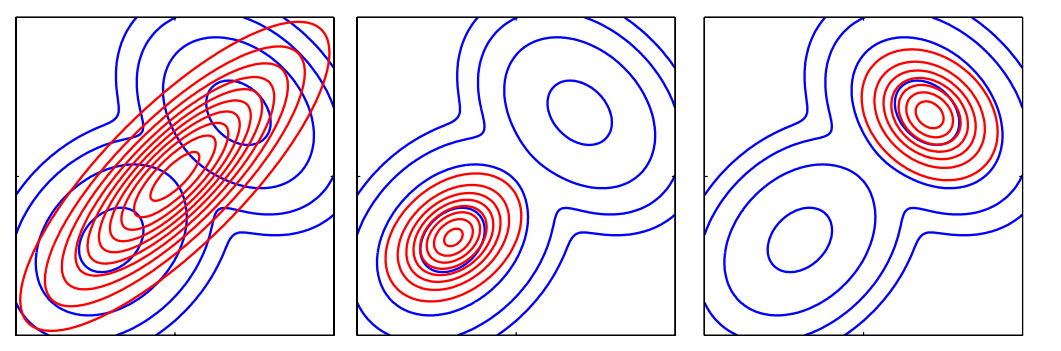
\includegraphics[width=\textwidth]{bishop.png}
\end{frame}


\begin{frame}{Использование вариационной нижней оценки}
\textbf{Для чего используют variational inference?}
\begin{itemize}
\item получение оценок Evidence;
\item получение оценок распределений моделей со скрытыми переменными (тематическое моделирование, снижение размерности).
\end{itemize}

\textbf{Зачем используют variational inference?}
\begin{itemize}
\item сводит задачу нахождения апостериорной вероятности к методам оптимизации;
\item проще масштабируется, чем аппроксимация Лапласа;
\item проще в использовании, чем сэмплирующие методы.
\end{itemize}
\textbf{Variational Inference может давать сильно заниженную оценку.}
\end{frame}


\section{Получение оценок для порождающих моделей}
\begin{frame}{Пример: автокодировщик}
Автокодировщик --- модель снижения размерности:
$$
	\mathbf{H} = \boldsymbol{\sigma}(\mathbf{W}_e \mathbf{X}),
$$
$$
	||\boldsymbol{\sigma}(\mathbf{W}_d\mathbf{H}) - \mathbf{X}||_2^2 \to \min.
$$

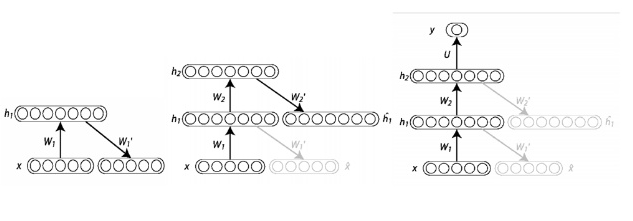
\includegraphics[width=\textwidth]{bengio.png}
\end{frame}



\begin{frame}{Вариационный автокодировщик}
\begin{columns}[T]
\begin{column}{.65\textwidth}
Пусть объекты выборки $\mathbf{X}$ порождены при условии скрытой переменной $\mathbf{h} \sim \mathcal{N}(\mathbf{0}, \mathbf{I})$:
$$
\mathbf{x} \sim p(\mathbf{x}|\mathbf{h}, \mathbf{w}).
$$
$p(\mathbf{h}|\mathbf{x}, \mathbf{w})$ --- неизвестно.

Будем максимизировать вариационную оценку правдоподобия выборки:
$$
\text{log}p(\mathbf{x}|\mathbf{w}) \geq \mathsf{E}_{q_\phi(\mathbf{h}|\mathbf{x})}\text{log}~p(\mathbf{x}|\mathbf{h}, \mathbf{w}) - D_\text{KL}(q_\phi(\mathbf{h}|\mathbf{x})||p(\mathbf{h})) \to \max.
$$

Распределения $q_\phi(\mathbf{h}|\mathbf{x})$ и $p(\mathbf{x}|\mathbf{h}, \mathbf{w})$ моделируются нейросетью:
$$
q_\phi(\mathbf{h}|\mathbf{x}) \sim \mathcal{N}(\boldsymbol{\mu}_\phi(\mathbf{x}),\boldsymbol{\sigma}_\phi^2(\mathbf{x})), 
$$
$$
p(\mathbf{x}|\mathbf{h}, \mathbf{w}) \sim \mathcal{N}(\boldsymbol{\mu}_w(\mathbf{h}),\boldsymbol{\sigma}_w^2(\mathbf{h})),
$$
где функции $\boldsymbol{\mu}$,$\boldsymbol{\sigma}$ --- выходы нейросети.\\
\end{column}%
\hfill%
\begin{column}{.25\textwidth}
\begin{figure}
  \centering
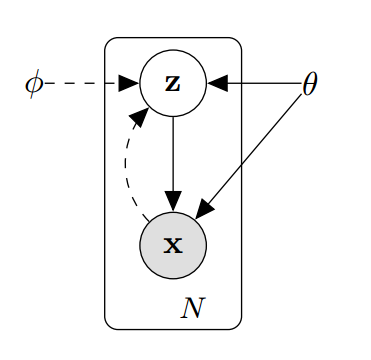
\includegraphics[width=\textwidth]{graph.png}
\end{figure}
\end{column}
\end{columns}
\end{frame}

\begin{frame}{Вариационный автокодировщик: evidence}

Оценка evidence получается двойным применением вариационной техники:
$$
\text{log}~p(\mathbf{X}|\mathbf{f}) \geq \mathsf{E}_{q_\mathbf{w}} \text{log}\hat{p}(\mathbf{x}|\mathbf{w}) + \text{log}~p(\mathbf{w}|\mathbf{f}) - \text{log}~q(\mathbf{w}),
$$
где $q_\mathbf{w}$ --- распределение, аппроксимирующее $p(\mathbf{w}|\mathbf{x}, \mathbf{f})$, $ \text{log}\hat{p}(\mathbf{x}|\mathbf{w})$ --- вариационная оценка правдоподобия выборки.

Для оптимизации вариационных параметов применяется следующая параметризация:
$$
\hat{\mathbf{w}} = \boldsymbol{\mu}_\mathbf{w} + \boldsymbol{\sigma}_{\mathbf{w}}\odot \boldsymbol{\epsilon}_1,\quad \hat{\mathbf{h}} = \boldsymbol{\mu}_\mathbf{h} + \boldsymbol{\sigma}_\mathbf{h}(\mathbf{h})\odot \boldsymbol{\epsilon}_2, 
$$
$$
\boldsymbol{\epsilon}_1, \boldsymbol{\epsilon}_2 \sim \mathcal{N}(\mathbf{0}, \mathbf{I}).
$$

\end{frame}
\section{Получение оценок для разделяющих моделей}
\begin{frame}{Разделяющие модели: правдоподобие}
Пусть $q \sim \mathcal{N}(\boldsymbol{\mu}_q, \mathbf{A}_q).$\\
Тогда вариационная оценка имеет вид:
$$
\int_{\mathbf{w}} q(\mathbf{w})\text{log}~{p(\mathbf{Y}|\mathbf{X},\mathbf{w},\mathbf{f})} d \mathbf{w} + D_\text{KL}\bigl(q (\mathbf{w} )|| p (\mathbf{w}|\mathbf{f})\bigr) \simeq
$$
$$
\sum_{i=1}^m \text{log}~p(\mathbf{y}_i|\mathbf{x}_i, \mathbf{w}_i) + D_\text{KL}\bigl(q (\mathbf{w} )|| p (\mathbf{w}|\mathbf{f})\bigr) \to \max_{\mathbf{A}_q, \boldsymbol{\mu}_q},
$$

В случае, если априорное распределение параметров $p(\mathbf{w}|\mathbf{f})$ является нормальным: 
$$
p(\mathbf{w}|\mathbf{f}) \sim \mathcal{N}(\boldsymbol{\mu}, \mathbf{A}),
$$
дивергенция $D_\text{KL}\bigl(q (\mathbf{w} )|| p (\mathbf{w}|\mathbf{f})$ вычисляется аналитически:
$$
D_\text{KL}\bigl(q (\mathbf{w} || p (\mathbf{w}|\mathbf{f})\bigr) = \frac{1}{2} \bigl( \text{tr} (\mathbf{A}^{-1}\mathbf{A}_q) + (\boldsymbol{\mu} - \boldsymbol{\mu}_q)^\text{T}\mathbf{A}^{-1}(\boldsymbol{\mu} - \boldsymbol{\mu}_q) - n +\text{ln}~|\mathbf{A}| - \text{ln}~|\mathbf{A}_q| \bigr).
$$
\end{frame}




\begin{frame}{Градиентный спуск для оценки правдоподобия}
Проведем оптимизацию нейросети в режиме мультистарта из $r$ различных начальных приближений $\mathbf{w}_1, \dots, \mathbf{w}_r$ с использованием градиентного спуска:
\[
\mathbf{w}' = \mathbf{w} - \alpha  \nabla \sum_{\mathbf{x} \in \mathbf{X}} \text{log}~p(\mathbf{x},\mathbf{w}|\mathbf{f}) = \sum_{\mathbf{x} \in \mathbf{X}} \text{log}~p(\mathbf{x}|\mathbf{w}, \mathbf{f}) p(\mathbf{w}|\mathbf{f}).
\]

Векторы параметров $\mathbf{w}_1,\dots,\mathbf{w}_r$ соответствуют некоторому скрытому распределению $q(\mathbf{w})$.

\end{frame}

\begin{frame}{Энтропия}
Формулу вариационной оценки можно переписать с использованием энтропии:
$$\text{log}~p(\mathbf{X}|\mathbf{f}) \geq 
\int_{\mathbf{w}} q(\mathbf{w})\text{log}~\frac{p(\mathbf{X},\mathbf{w}|\mathbf{f})}{q(\mathbf{w})}d\mathbf{w} = 
$$
$$
\mathsf{E}_{q(\mathbf{w)}}[\text{log~}p (\mathbf{X}, \mathbf{w}| \mathbf{f})] - \mathsf{S}({q(\mathbf{w)}}),
$$
где $\mathsf{S}({q(\mathbf{w)}})$ --- энтропия:
$$
\mathsf{S}({q(\mathbf{w)}}) = - \int_{\mathbf{w}} q(\mathbf{w})\text{log}~q(\mathbf{w})d\mathbf{w}.  	
$$


\end{frame}


\begin{frame}{Градиентный спуск для оценки правдоподобия}
При достаточно малой длине шага оптимизации $\alpha$ разность энтропии на различных шагах оптимизации вычисляется как:
\[
\mathsf{S}(q'(\mathbf{w})) -  \mathsf{S}(q(\mathbf{w}))  \simeq  \frac{1}{r}\sum_{g=1}^r \bigl(-\alpha \text{Tr}[\mathbf{H}(\mathbf{w}'^g)] - \alpha^2 \text{Tr}[\mathbf{H}(\mathbf{w}'^g)\mathbf{H}(\mathbf{w}'^g)]  \bigr).
\]

Итоговая оценка на шаге оптимизации $\tau$:
$$
\text{log}~\hat{p}(\mathbf{Y}|\mathbf{X}, \mathbf{f}) \sim \frac{1}{r} \sum_{g = 1}^r L(\mathbf{w}^g_\tau, \mathbf{X}, \mathbf{Y})  + \mathsf{S}(q^0(\mathbf{w})) + \frac{1}{r}\sum_{b=1}^\tau\sum_{g=1}^r \bigl(-\alpha \text{Tr}[\mathbf{H}(\mathbf{w}_b^g)] - \alpha^2 \text{Tr}[\mathbf{H}(\mathbf{w}_b^g)\mathbf{H}(\mathbf{w}_b^g)]  \bigr),
$$
$\mathbf{w}_b^g$ --- вектор параметров старта $g$ на шаге $b$, $\mathsf{S}(q^0(\mathbf{w}))$ --- начальная энтропия.
\end{frame}
\begin{frame}{Переобучение}
Градиентный спуск не минимизирует дивергенцию $\text{KL}(q(\mathbf{w})||p(\mathbf{w}| \mathbf{X}))$. При приближении к моде распределения снижается оценка Evidence, что интерпретируется как переоубчение модели.

\begin{figure}
  \centering
  \subfloat[Схождение распределения к моде]{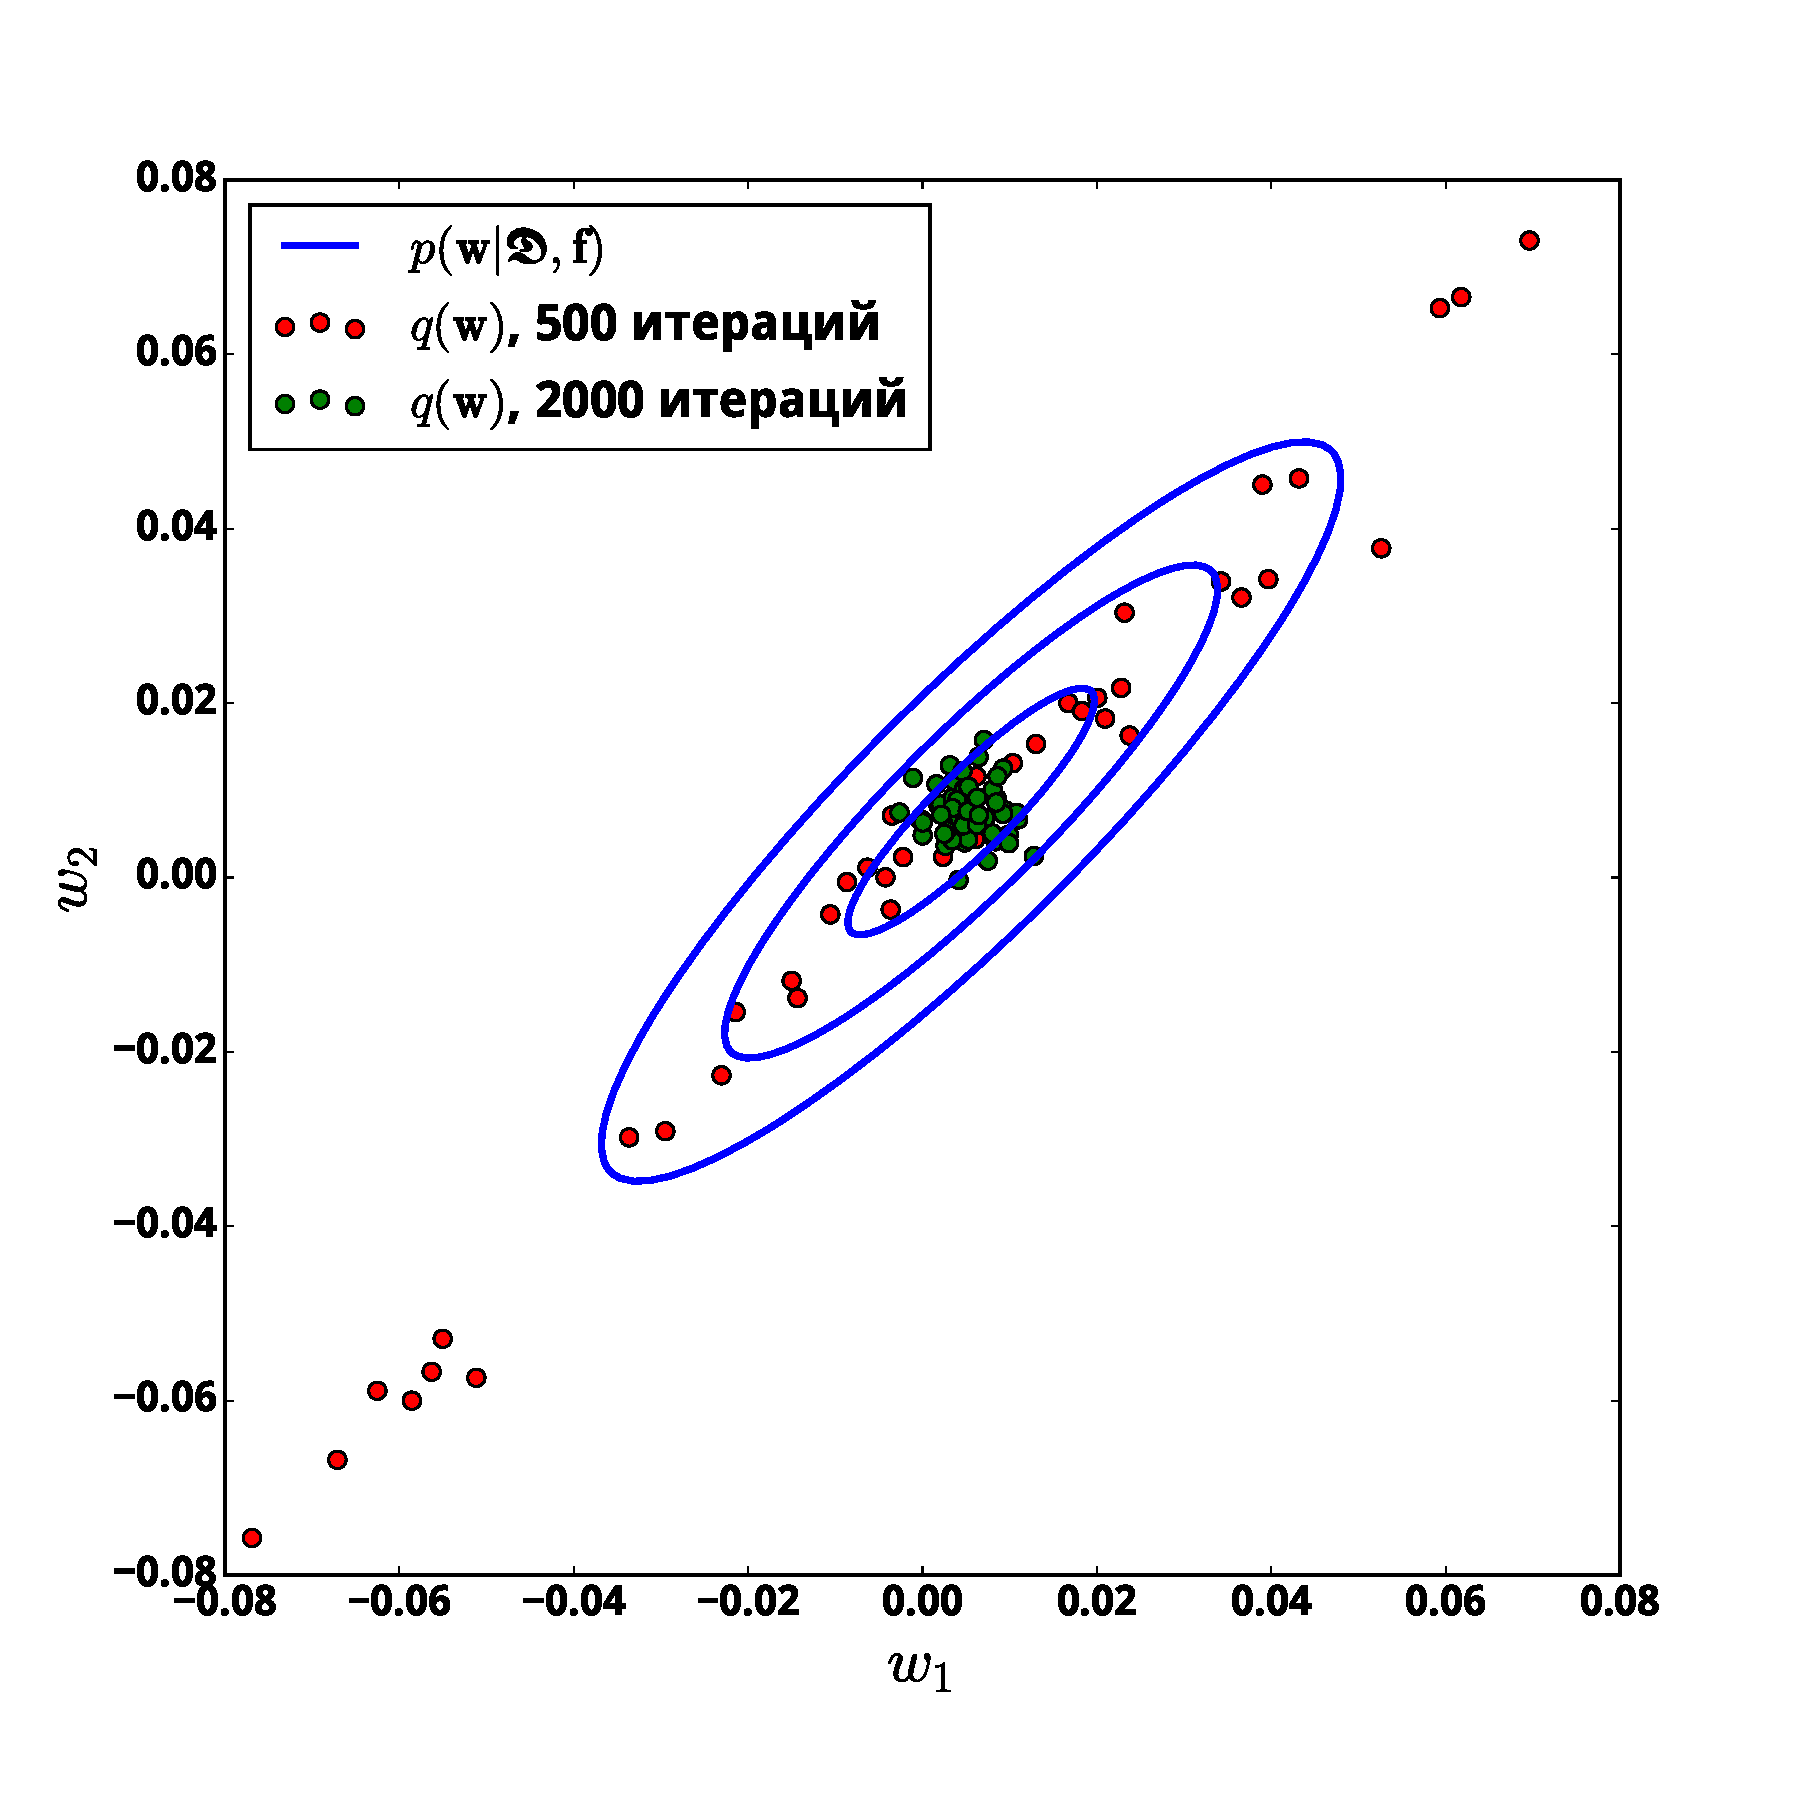
\includegraphics[width=0.35\textwidth]{sgd_estimate.pdf}} 
 \subfloat[Оценка начала переобучения]{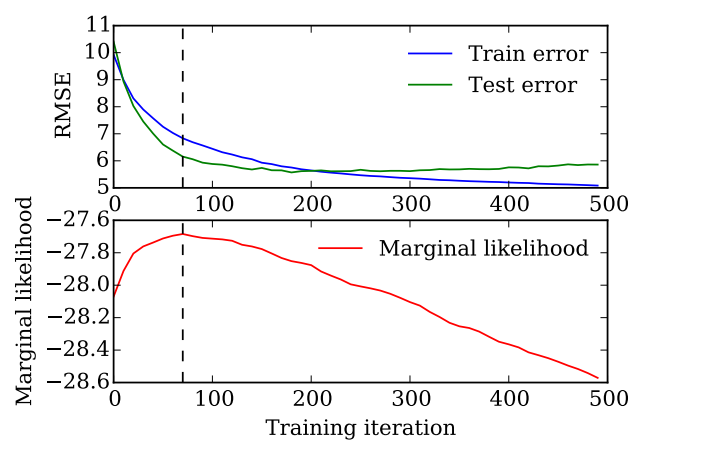
\includegraphics[width=0.4\textwidth]{overfit.png}}
\label{fig:1}\qquad
\end{figure}
\end{frame}

\begin{frame}
\frametitle{Стохастическая динамика Ланжевина}
Модификация стохастического градиентного спуска:
\[
	\Delta \mathbf{w} = \alpha \nabla (\text{log}p(\mathbf{w})+\frac{m}{\hat{m}}\text{log}p(\hat{\mathbf{X}}|\mathbf{w}))  \textcolor{red}{+ \epsilon, \quad   \textcolor{red}{\epsilon \sim  \mathcal{N}({0},{\frac{\alpha}{2}})}}
\]
где $\hat{m}$ --- размер подвыборки,  $\hat{\mathbf{X}} \subset \mathbf{X}$ --- подвыборка, шаг оптимизации $\alpha$ изменяется с количеством итераций:
\[
	\sum_{\tau=1}^\infty \alpha_\tau = \infty, \quad \sum_{\tau=1}^\infty \alpha_\tau^2 < \infty.
\]
\textbf{Утверждение~[Welling, 2011].} Распределине $q^\tau(\mathbf{w})$ сходится к апостериорному распределению $p(\mathbf{w} | \mathbf{X},\mathbf{f})$.


Изменение энтропии с учетом добавленного шума:
\[
\hat{\mathsf{S}}\bigl(q^\tau(\mathbf{w})\bigr)   \geq \frac{1}{2}|\mathbf{w}|\text{log}\bigl(\text{exp}(\frac{2\mathsf{S}(q^\tau(\mathbf{w}))}{|\mathbf{w}|}) + \text{exp}(\frac{2\mathsf{S}( \epsilon)}{|\mathbf{w}|})\bigr).
\]

\end{frame}


\begin{frame}
\frametitle{Стохастическая динамика Ланжевина}
Распределения параметров после 2000 итераций:
\begin{figure}[h]
\centering
\subfloat[]{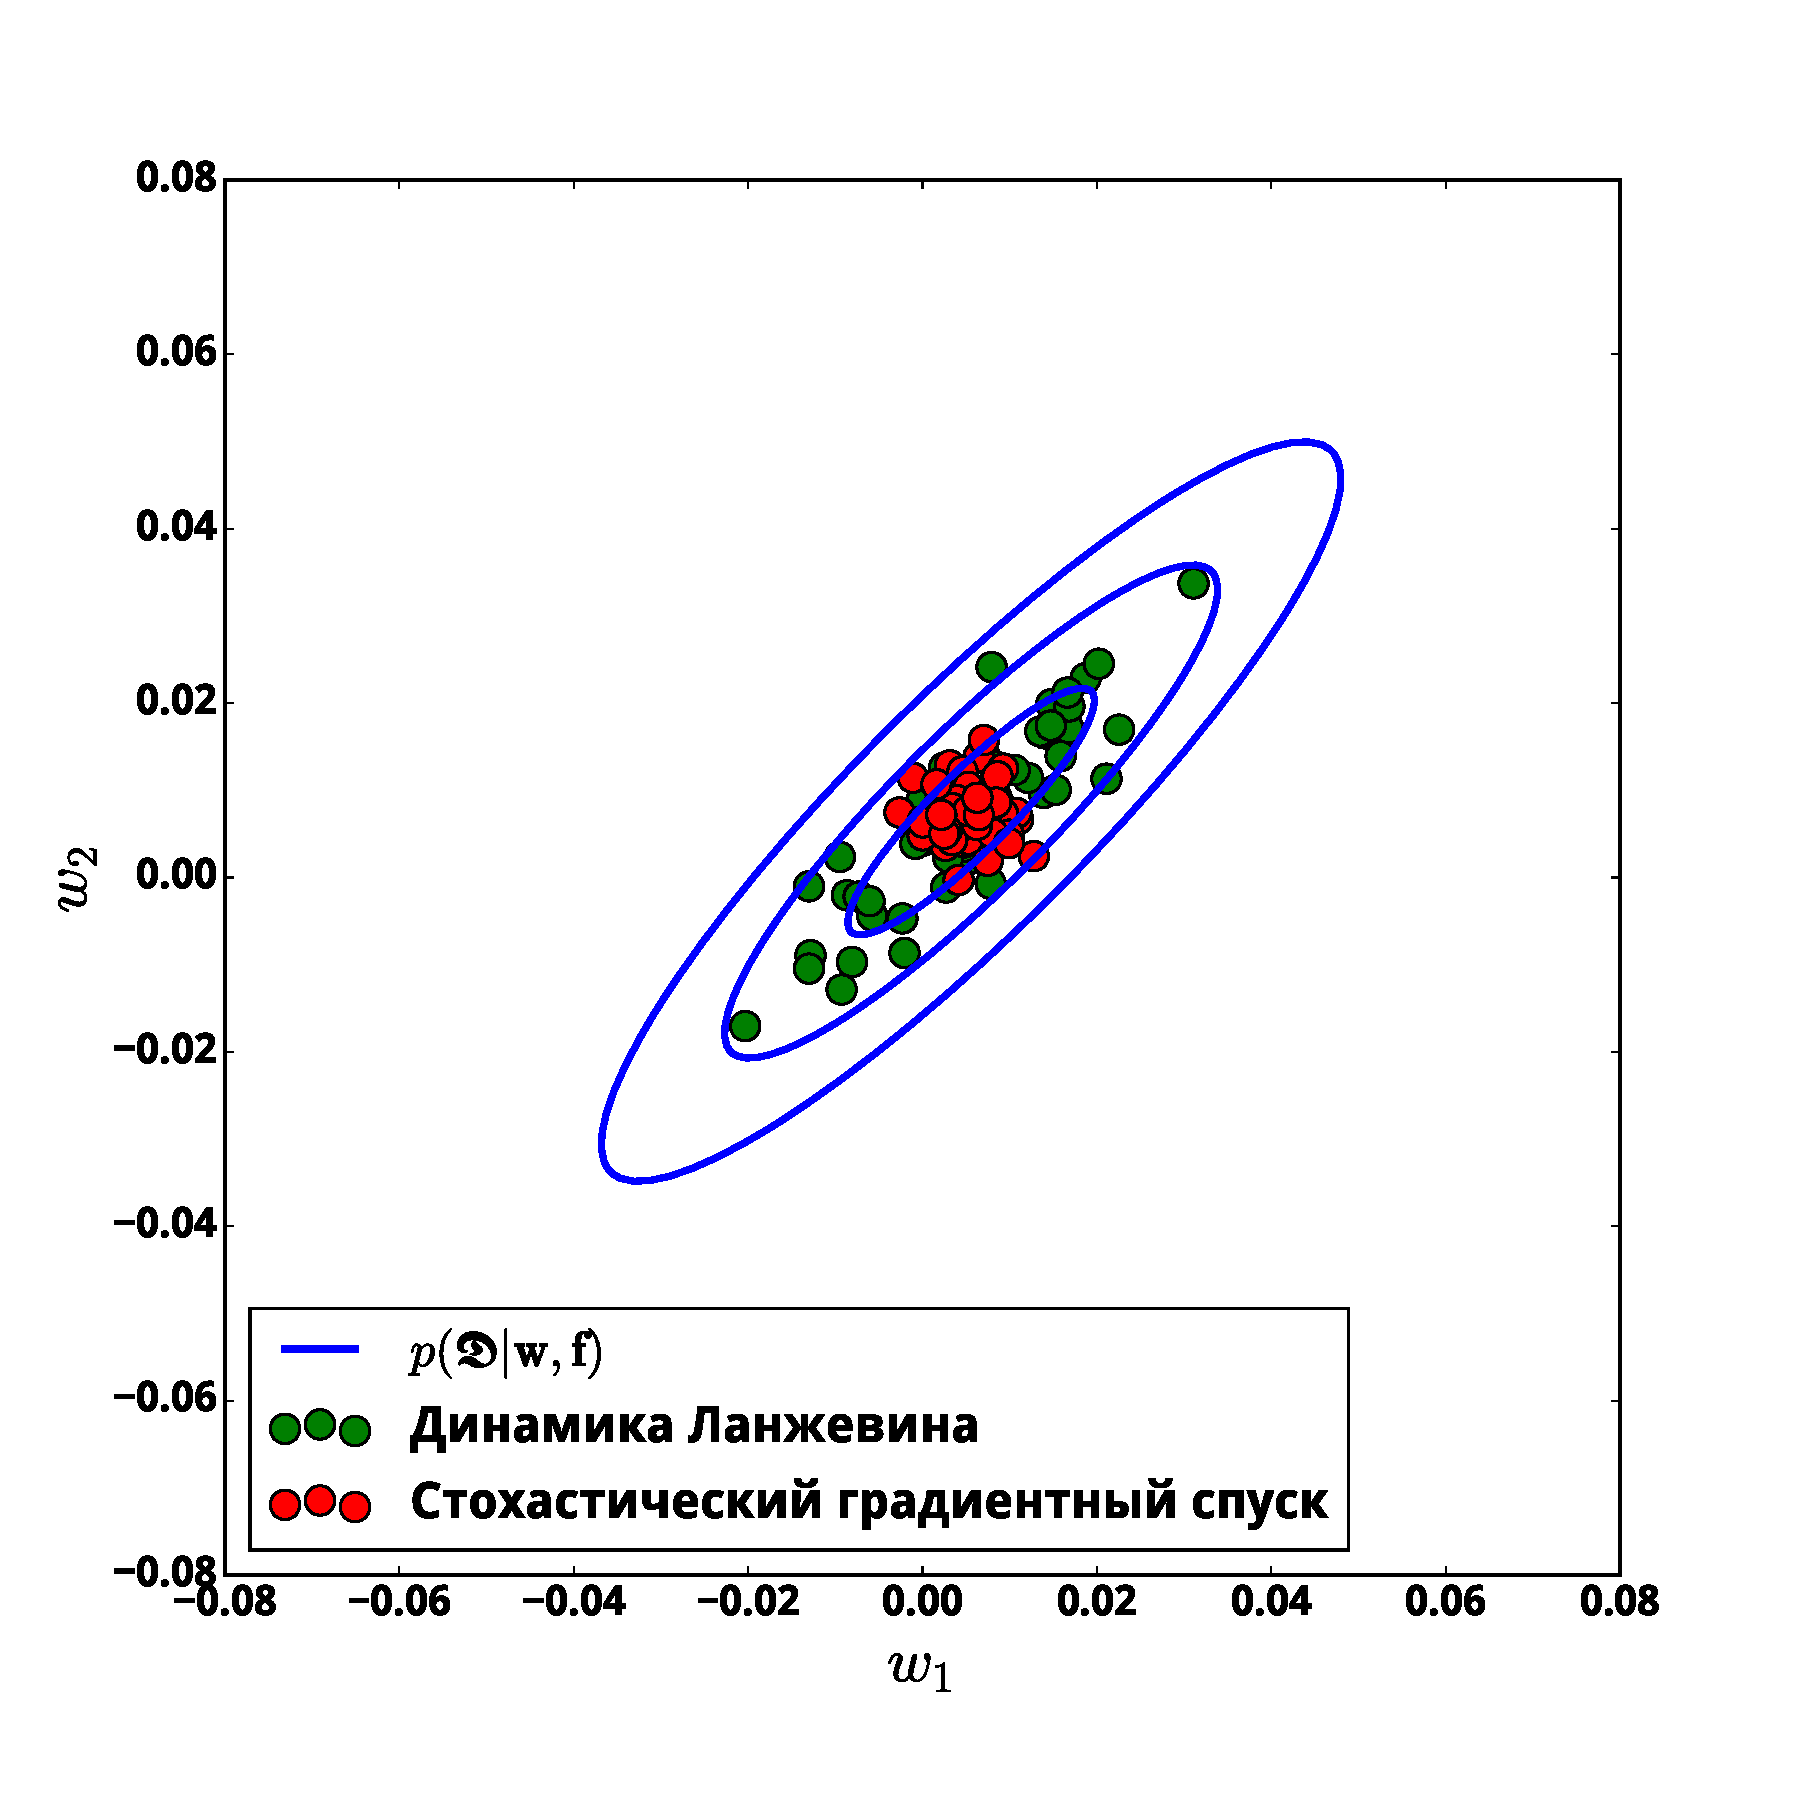
\includegraphics[width=0.45\textwidth]{./langevin_estimate.pdf}}
\end{figure}

\end{frame}

\begin{frame}{Пример: выбор константы регуляризации}
Выборка MNIST, 50 нейронов на скрытом слое.

\begin{figure}
  \centering
  \subfloat[Кросс-валидация]{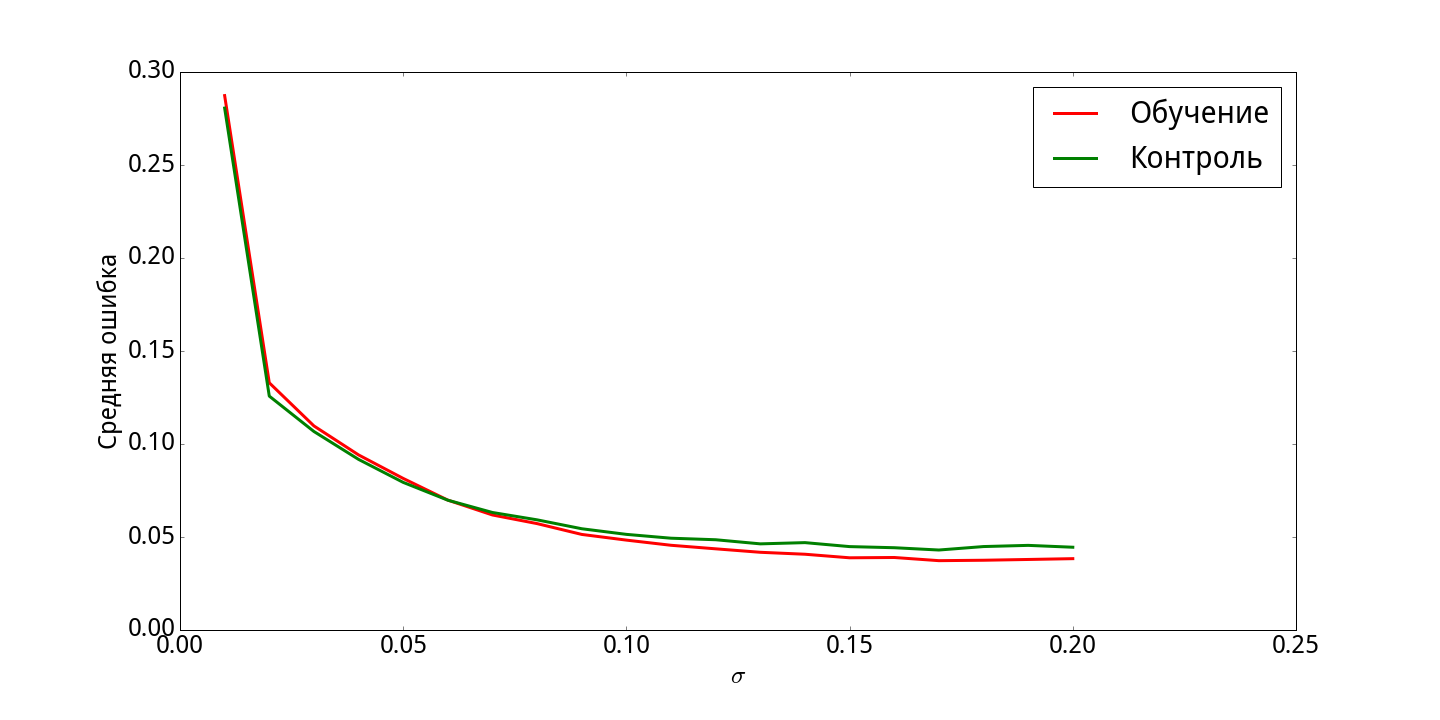
\includegraphics[width=0.5\textwidth]{sgd2.png}} 
 \subfloat[Оценка Evidence]{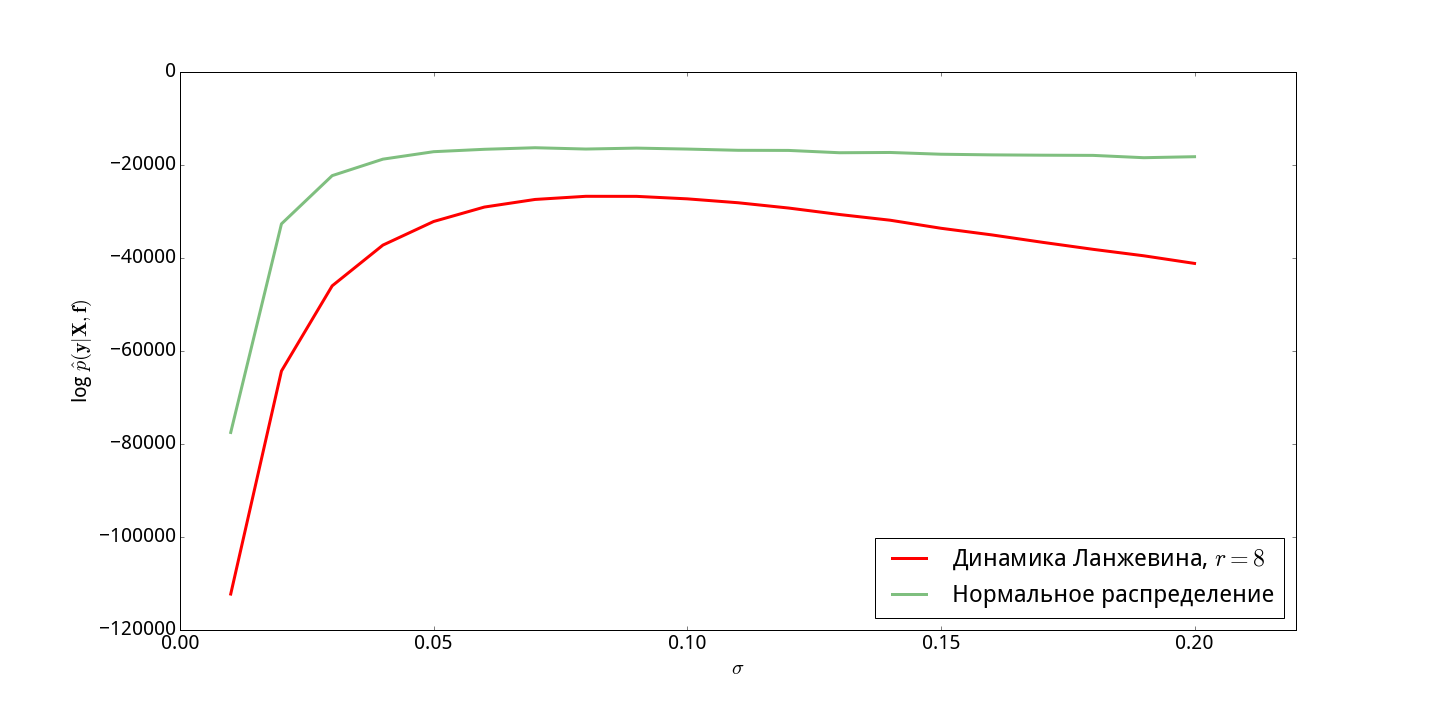
\includegraphics[width=0.5\textwidth]{mnist_evidence2.png}}
\label{fig:1}\qquad
\end{figure}

\end{frame}
\begin{frame}{Пример: ранняя остановка}
Выборка Boston, 50 нейронов на скрытом слое.


\begin{figure}
  \centering
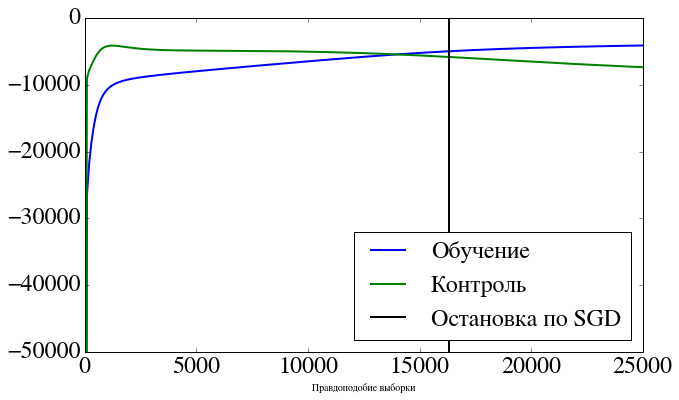
\includegraphics[width=0.75\textwidth]{stop.png}
\end{figure}


\end{frame}


\section{Выбор модели глубокого обучения}

\begin{frame}
\frametitle{Выбор моделей: Graves, 2011}
\textbf{Априорное распределение:} $p(\mathbf{w}|\sigma) \sim \mathcal{N}(\boldsymbol{\mu}, \sigma \mathbf{I}).$\\
\textbf{Вариационное распределение:} $q (\mathbf{w}) \sim \mathcal{N}(\boldsymbol{\mu}_q, \sigma_q \mathbf{I}).$\\
Жадная оптимизация гиперпараметров:
\[
	\boldsymbol{\mu} = \hat{\mathsf{E}} \mathbf{w},
\quad
	\sigma = \hat{\mathsf{D}} \mathbf{w}.
\]

Прунинг параметра ${w}_i$ определяется относительной плотностью:
\[
	\frac{q(\mathbf{0})}{q(\boldsymbol{\mu}_{i,q})}  = \text{exp}(-\frac{\mu_i^2}{2\sigma_i^2}).
\]
\end{frame}


\begin{frame}
\frametitle{Выбор моделей: Graves, 2011}
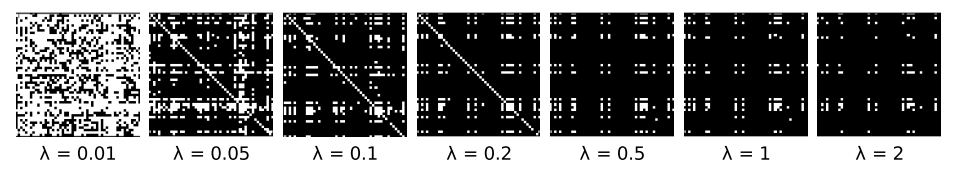
\includegraphics[width=\textwidth]{graves.png}
\end{frame}


\begin{frame}
\frametitle{Выбор моделей: Maclaurin, Duvenaud, Adams 2015}
Оптимизация гиперпараметров производится во внешнем цикле градиентными методами.\\
\textbf{Плюсы:}
\begin{enumerate}
\item Позволяет производить оптимизацию по произвольной дифференцируемой функции потерь.
\item Количество гиперпараметров неограничено.
\end{enumerate}
\textbf{Минусы:}
\begin{enumerate}
\item Сложно реализуется технически.
\item Появляются гиперпараметры внешнего цикла оптимизации
\end{enumerate}

\end{frame}


\begin{frame}
\frametitle{Выбор моделей: Optimal Brain Damage}
Разложим функцию потерь в окрестности точки минимума:
\[
	L (\mathbf{w} + \Delta \mathbf{w}) = L (\mathbf{w})  + \frac{\partial{L}}{\partial{\mathbf{w}}}^\text{T}\Delta\mathbf{w} + 0.5\Delta\mathbf{w}^\text{T}\mathbf{H}\Delta\mathbf{w} + o(|\mathbf{w}|^3).
\]

Выбор параметра для удаления:
\[
	i = \text{argmin} \Delta\mathbf{w}^\text{T}\mathbf{H}\Delta\mathbf{w}
\]
при условии:
\[
	\Delta\mathbf{w}_i + w_i = 0.
\]
\end{frame}

\begin{frame}
\frametitle{Выбор моделей: Попова,  Стрижов, 2015}
\textbf{Критерии прореживания и наращивания сети}
\begin{itemize}
\item Критерий оптимального проржеивания --- OBD.
\item Критерий последовательного прореживания:  $i = \text{argmin} L(\mathbf{f}/{w}_i)$.
\item Критерий устойчивого прореживания --- основан на анализе матрицы ковариаций параметров.
\item Критерий последовательного наращивания:  $i = \text{argmin} L(\mathbf{f} \cup {w}_i)$.
\end{itemize}
\begin{figure}
\centering
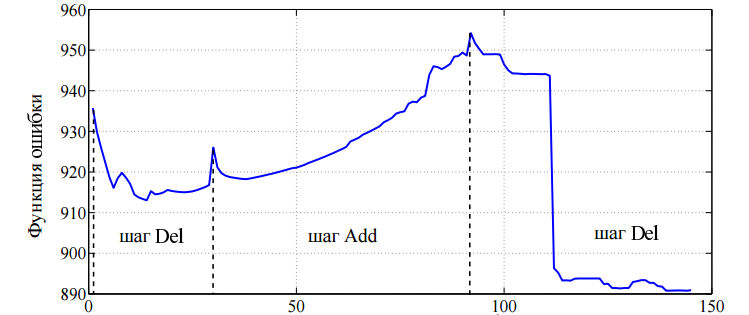
\includegraphics[width=0.7\textwidth]{adddel.png}
\end{figure}
\end{frame}


\begin{frame}
\frametitle{Используемые материалы}
\begin{enumerate}
\item David J. C. MacKay, Information Theory, Inference \& Learning Algorithms
\item Peter Grunwald, A tutorial introduction to the minimum description length principle
\item Kuznetsov M.P., Tokmakova A.A., Strijov V.V. Analytic and stochastic methods of structure parameter estimation
\item Christopher Bishop, Pattern Recognition and Machine Learning
\item Yoshua Bengio, Pascal Lamblin, Dan Popovici, Hugo Larochelle, Greedy Layer-Wise Training of Deep Networks
\item Diederik P Kingma, Max Welling, Auto-Encoding Variational Bayes
\item Dougal Maclaurin, David Duvenaud, Ryan P. Adams, Early Stopping is Nonparametric Variational Inference
\item Max Welling, Yee Whye Teh, Bayesian Learning via Stochastic Gradient Langevin Dynamics
\end{enumerate}
\end{frame}

\begin{frame}
\frametitle{Используемые материалы}
\begin{enumerate}
\item A. Graves, Practical Variational Inference for Neural Networks
\item D. Maclaurin, D. Duvenaud, R. P. Adams, Gradient-based Hyperparameter Optimization through Reversible Learning
\item Y. Le Cun, J. S. Denker, S. A. Solia, Optimal Brain Damage 
\item М. С. Попова, В. В. Стрижов, Выбор оптимальной модели классификации физической активности по измерениям акселерометра
\end{enumerate}
\end{frame}

\end{document}

